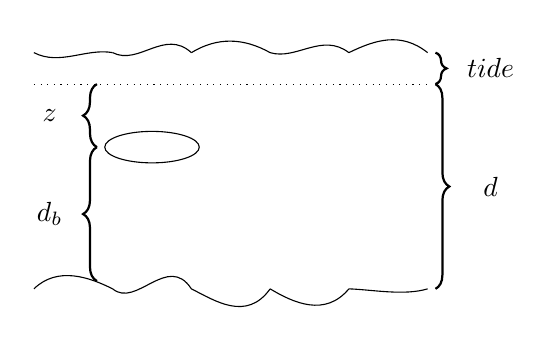
\begin{tikzpicture}
%Water surface
\draw (0,0) .. controls (0.33,-0.17) and (0.66,0.06) .. (1,0);
\draw (1,0) .. controls (1.33,-0.17) and (1.66,0.31) .. (2,0);
\draw (2,0) .. controls (2.33,0.2) and (2.66,0.19) .. (3,0);
\draw (3,0) .. controls (3.33,-0.1) and (3.66,0.26) .. (4,0);
\draw (4,0) .. controls (4.33,0.16) and (4.66,0.27) .. (5,0);

\draw[dotted] (0,-0.4) -- (5,-0.4);

%AUV
%\draw[rotate=25] (1,-1.7) ellipse (0.6 and 0.2);
\draw (1.5,-1.2) ellipse (0.6 and 0.2);

\draw (0,-3) .. controls (0.3,-2.71) and (0.7,-2.85) .. (1,-3);
\draw (1,-3) .. controls (1.3,-3.25) and (1.7,-2.54) .. (2,-3);
\draw (2,-3) .. controls (2.3,-3.15) and (2.7,-3.42) .. (3,-3);
\draw (3,-3) .. controls (3.3,-3.18) and (3.7,-3.36) .. (4,-3);
\draw (4,-3) .. controls (4.3,-3.01) and (4.7,-3.09) .. (5,-3);

%Curli braces
\draw [decorate, decoration={brace, amplitude=5pt, mirror}, thick] (5.1, -3)  -- (5.1, -0.4) 
 node[label, midway, xshift=7mm] {$d$};
\draw [decorate, decoration={brace, amplitude=4pt, mirror}, thick] (5.1, -0.4)  -- (5.1, 0) 
 node[label, midway, xshift=7mm] {$tide$};
 
\draw [decorate, decoration={brace, amplitude=5pt, mirror}, thick] (0.8, -0.4)  -- (0.8, -1.2) 
 node[label, midway, xshift=-6mm] {$z$};
\draw [decorate, decoration={brace, amplitude=5pt, mirror}, thick] (0.8, -1.2)  -- (0.8, -2.9) 
 node[label, midway, xshift=-6mm] {$d_b$};

\end{tikzpicture}